\section{Day 4}
\begin{tabular}{|c|c|}
Date: & 10.10.1987 \\
\end{tabular}
\subsection{1st session: Review of training}
The datamanagers from different facilities reviewed their previos training. See email from Gloria for more information.
Wheres the map? (Because they removed it.)\\
Inser chart list maybe to long.\\
Why is the top border gone in gis? (Problem solved)\\
Wheres the back button? (Found it!)\\
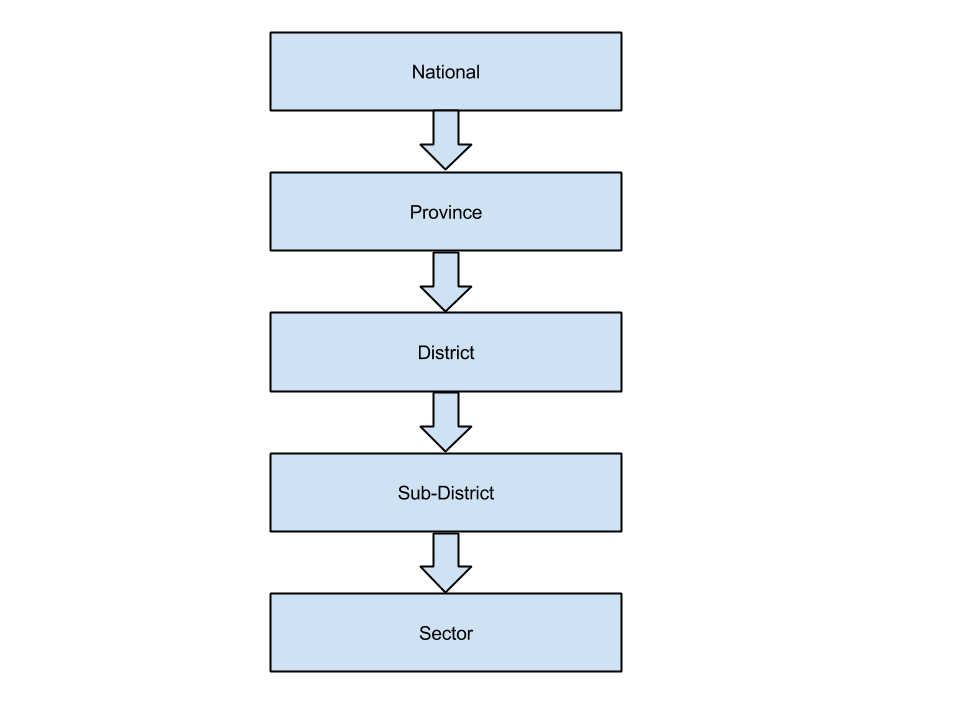
\includegraphics[width=15cm]{appendix/images/dhis2_map_categories}
\subsection{Meeting}
We talked a little bit here in order to get a better understanding of how they used the DHIS2. The consisted of me, Simen, Gloria, Adolf and three other data managers. It was a little difficult at first, but after a while I think we've got a pretty good understanding of it. They use DHIS2 for data analyses and for reporting data. Reporting data is done by the data manager at each health facility. Data analysing is used by monitoring and evaluation officer and head of community officers for decision making and strategic planning. \\
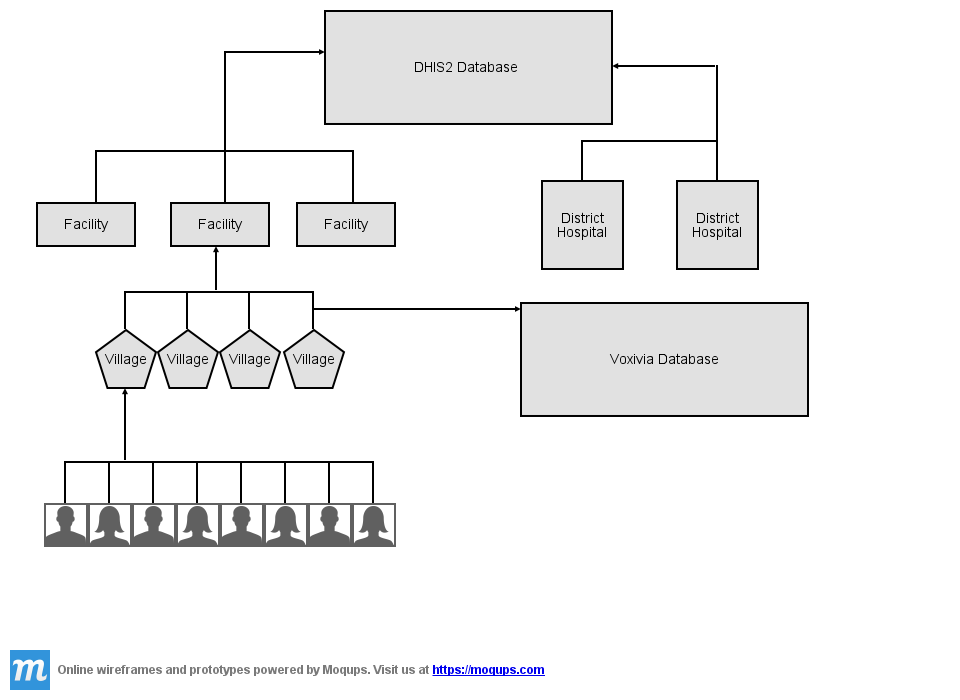
\includegraphics[width=15cm]{appendix/images/Dataflow} \\
The collecting of data starts in paper form. They are then gathered at each facility for reporting in the DHIS2 database. They have a seperate reporting system with voxivia. They still use this because they allow for more detailed information. If they use DHIS2 they have to track the reporting to the paperbased forms in order to get the ground details. Adolf mentioned that he would like a way to combine the data from the tracker and the aggregated data. This was a nice feature that they would like.
\subsection{Dinner}
Dinner was awsome!
\subsection{Second Session}
We then had a look at their presentations. We only stayed for one presentation. Then it was photo's. Thumbs up Simen!
